La elección sobre la metodología que se utiliza es crítica cuando se desarrolla un proyecto de software, debido esta sólo se realiza al inicio del proyecto. 

Existen muchas metodologías las cuales tienen amplia documentación y han probado ser eficientes para casos en específicos, los motivos por los cuales utilizar la metodología ágil Melé son:

\begin{itemize}
	\item Completa participación del cliente y prueba de funcionalidades para obtener retroalimentación.

	\item Se pueden obtener los cambios y adaptarse al proyecto en cada Sprint.

	\item Como la idea principal es realizar rendiciones y se han aclarado algunos requerimientos, mas no son todos, es que se esperaba que el proyecto aumente en el proceso de desarrollo. Es por esta incertidumbre que se escoge la metodología Melé, ya que ayuda al cliente y al equipo de trabajo a definir los requisitos del proyecto.
\end{itemize}

Pero dado a que la metodología esta diseñada para utilizarse en equipos de personas, esta se tuvo que ajustar cada rol con sus responsables a sólo un individuo, ya que la implementación del sistema esta bajo la responsabilidad a una persona.

En cuanto a la duración de cada Sprint, se determina como en tres semanas, tiempo relativamente razonable para realizar iteraciones de productos utilizables.

Para el desarrollo de cada Sprint, se utilizó utilizar la aplicación gratuita y Open Source Taiga, que es una plataforma de gestión de proyectos diseñadores ágiles.

Para comenzar a utilizar esta plataforma se deben registrar las historias de usuarios. Una ves realizado lo anterior, se proceden a crear los Sprint y por último se añaden las historias de usuarios a cada Sprint tal como se muestra en \textbf{Figura~\ref{fig: backlog}}.

\begin{figure}[h!]
	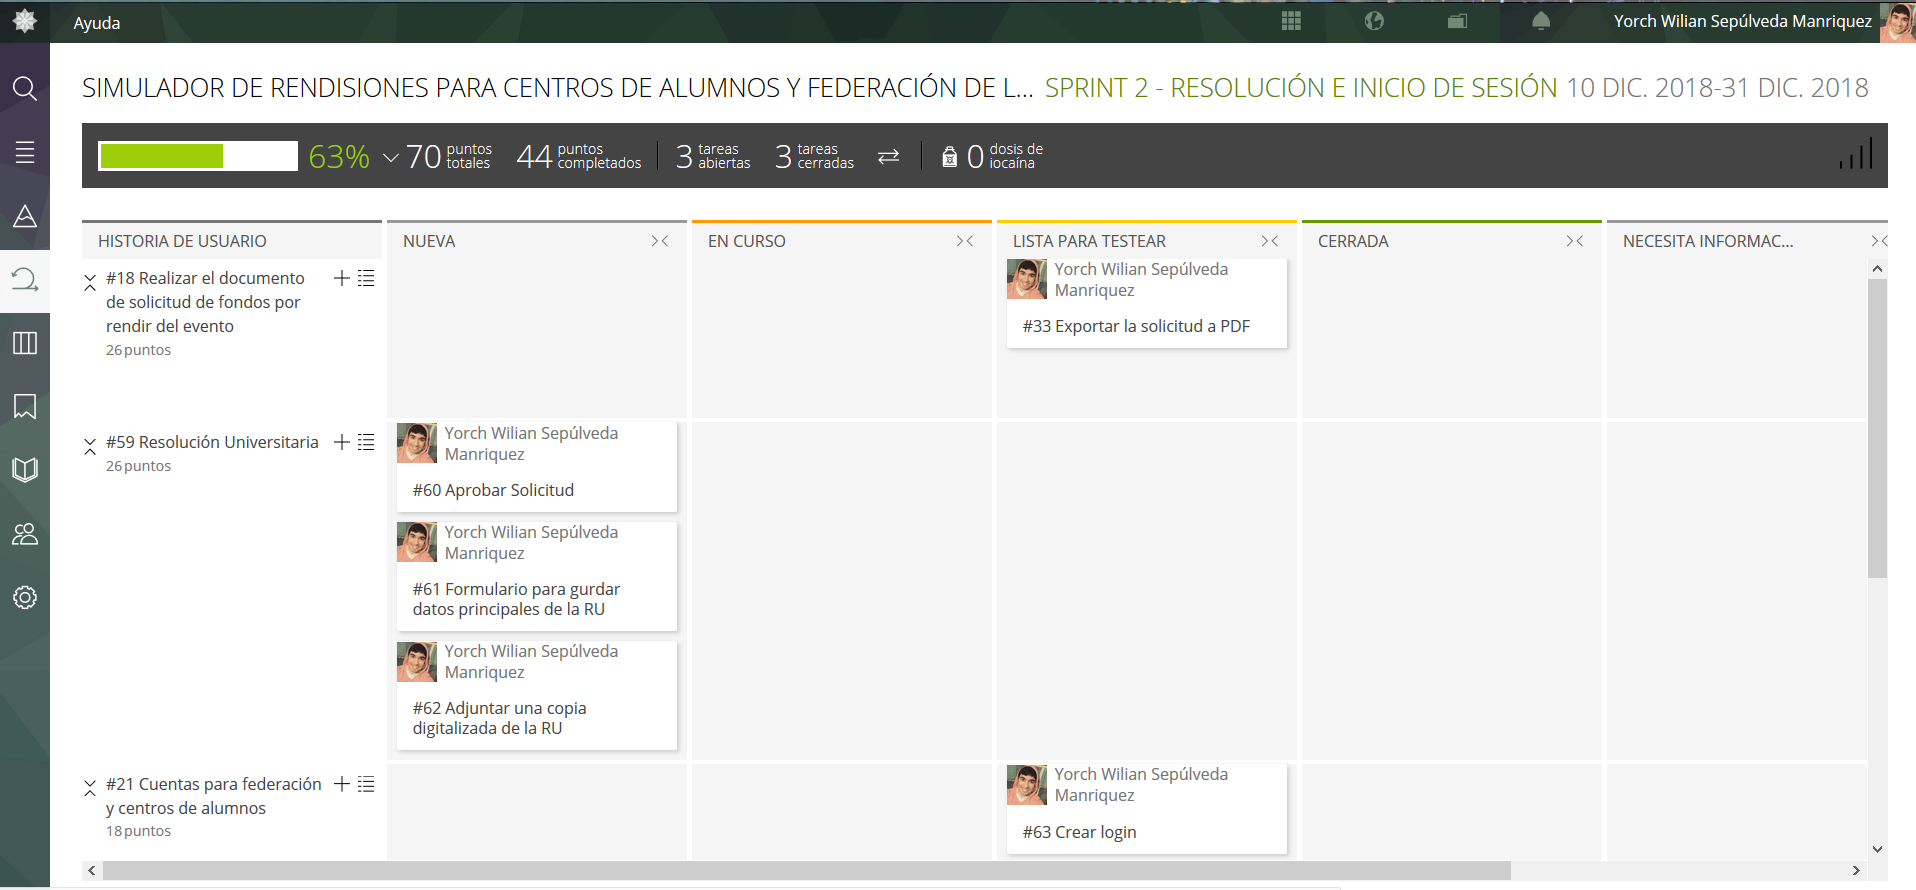
\includegraphics[width=\textwidth]{Imagenes/Kanban.png}
	\caption{\label{fig: backlog} Backlog.}
\end{figure}

Dentro de cada Sprint hay un Kanban, el cual ayuda a organizar el desarrollo de cada historia de usuario realizada en el Sprint Backlog, en donde divide el trabajo en pequeñas tarjetas o tickets.

Dado lo anterior es que se divide el proceso de trabajo en cinco columnas como se muestra en \textbf{Figura~\ref{fig: kanbanSprint}}, en donde se encuentran:

\begin{itemize}
	\item 	\begin{description}
				\item[Nueva:] Se ingresan pequeñas tarjetas o ticket de trabajo que ayudan a realizar el cumplimiento de la historia de usuario 
			\end{description}

	\item 	\begin{description}
				\item[En curso:] sección en donde se encuentran las tareas que se estan realizando
			\end{description}

	\item 	\begin{description}
			    \item[Lista para Testear:] columna en la que se encuentran las tareas terminadas y en proceso de aceptación
			\end{description}

	\item 	\begin{description}
				\item[Cerrada:] área en donde se encuentran las tareas que han sido finalizada y aceptadas.
			\end{description}
	
	\item 	\begin{description}
				\item[Necesita Información:] sección en donde se encuentran las tareas que no ha logrado culminarse debido a que falta información para su realización.
			\end{description}
\end{itemize}

\begin{figure}[h!]
	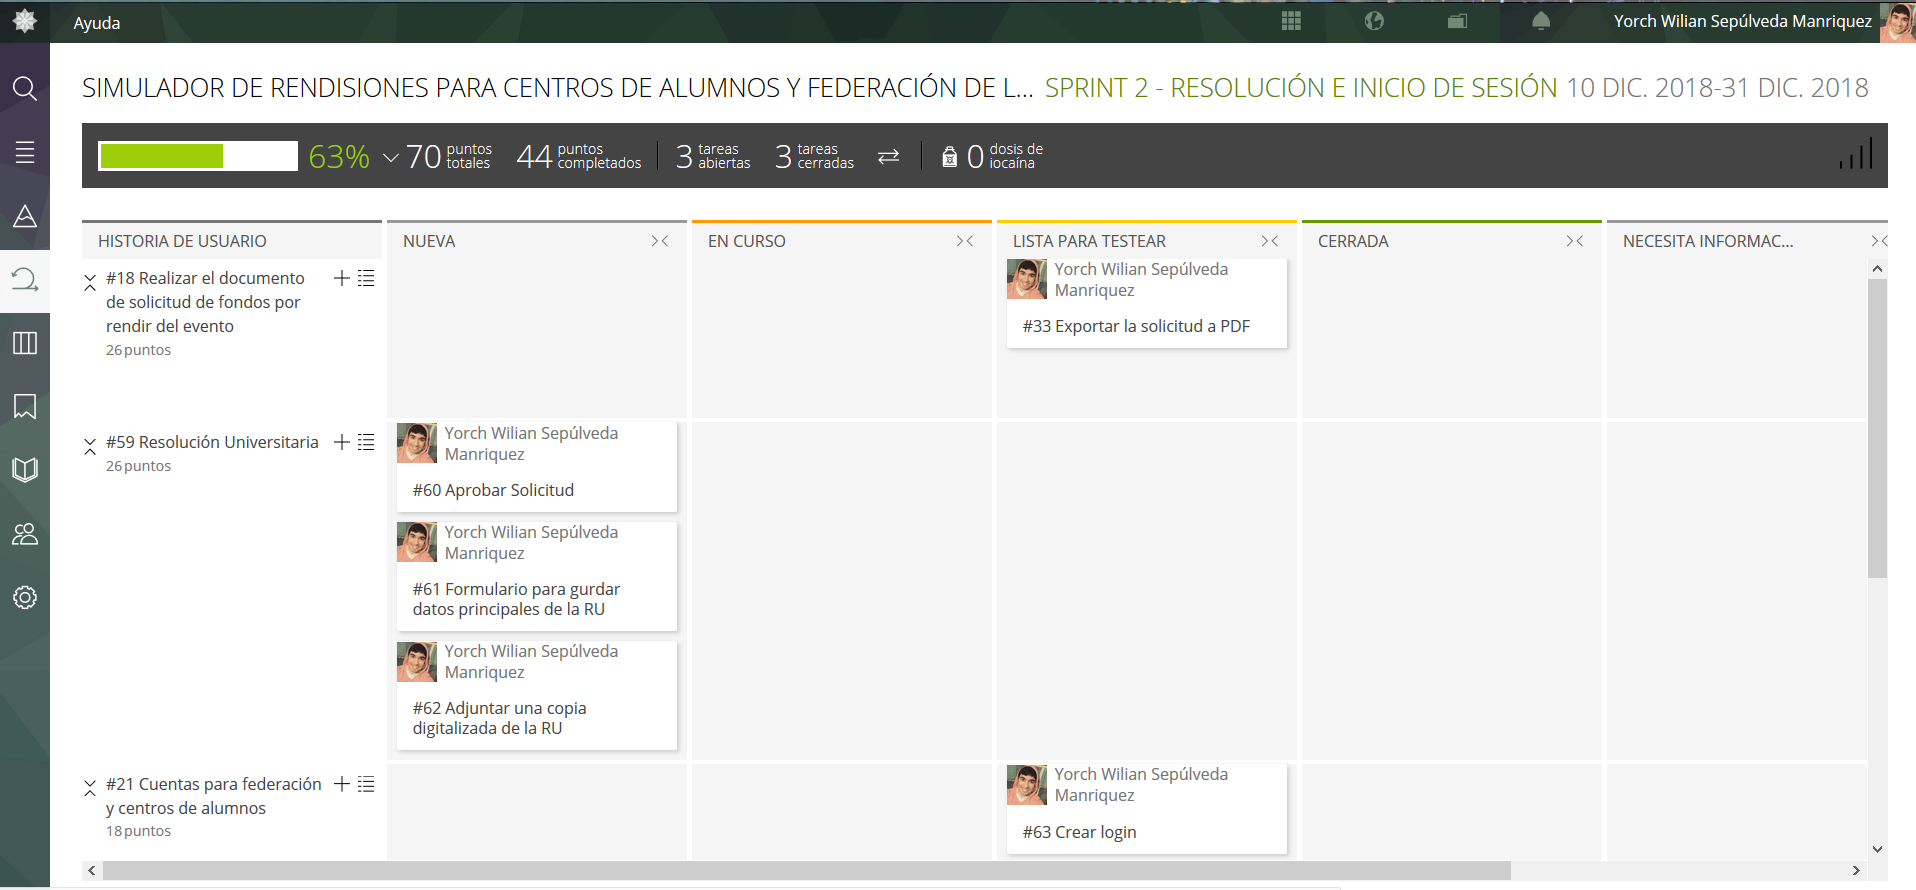
\includegraphics[width=\textwidth]{Imagenes/Kanban.png}
	\caption{\label{fig: kanbanSprint} Proceso de trabajo de un Sprint.}
\end{figure}